\documentclass{article}

\usepackage[a4paper,margin=2cm]{geometry}
\usepackage{array}
\usepackage{amsmath}
\usepackage{amsfonts}
\usepackage{fancyhdr}
\usepackage{tabularx}

\usepackage{tikz}
\usepackage{pgfplots}

\usepackage{enumitem}

\lhead{Name:}

\chead{Komplexe Zahlen $\mathbb{C}$}

\rhead{Datum: \hphantom{dd.MM.yyyy}}

\pagestyle{fancy}

\pgfplotsset{compat=1.18}

\begin{document}

    \large  

    \section{Komplexe Zahlen $\mathbb{C}$}

    %\subsection{Zahlbereichserweiterung}

\parbox{0.9\textwidth}{
    Ziel ist es Gleichungen wie $\mathbf{x^2 + 1 = 0}$ zu lösen.
    Man definiert dazu nun eine Einheit $\mathbf{i}$ mit der Eigenschaft $\mathbf{i^2 = -1}$.
    Für so eine Zahl ist nun jedoch kein Platz mehr in der Zahlengerade, 
    deshalb erweitert man die Zahlengerade mit den Komplexen Zahlen zu einer \textbf{Zahlenebene}.
    Somit sind die komplexen Zahlen eine \textbf{Erweiterung der Reellen Zahlen}.
    Dies wird auch \textbf{Zahl(en)bereichserweiterung} genannt
} 

\subsection{Komplexe Zahlen als Vektorraum}

\parbox{0.9\textwidth}
{
    Eine komplexe Zahl als Wertepaar kann mit einem Vektor im Vektorraum $\mathbb{R}^2$ verglichen werden,
    wobei auch Rechenarten, wie Addition und Multiplikation analog zur Vektoraddition und Vektormultiplikation sind.
    Der Vektorraum bei komplexen Zahlen hat wie der Vektorraum von $\mathbb{R}^2$ zwei Kooridnatenachsen.
    Dabei gibt die x-Achse den reelen Anteil und die y-Achse den imaginären Anteil der komplexen Zahl an.
    Für die Darstelling komplexer Zahlen wird die Gleichung 
    $\mathbf{z = \left(a; b\right) = a \cdot \left(1; 0\right) + b \cdot \left(0;1\right)}$ verwendet.
    Dabei ist das Wertepaar $\mathbf{\left(1; 0\right) = 1}$ als Einselement definiert, während das Wertepaar 
    $\mathbf{\left(0; 1\right) = i}$ angibt. Es ergibt sich also folgende Gleichung: 
    $\mathbf{z = a \cdot 1 + b \cdot i = a + bi}$.

    Eine komplexe Zahl $\mathbf{z}$ ist nun \textbf{ein Punkt} $\mathbf{\left(a;b\right)}$ auf der Zahlenebene,
    wobei $\mathbf{a}$ \textbf{die Reele und} $\mathbf{b}$ \textbf{die imaginäre Komponente der Zahl} $\mathbf{z}$ \textbf{ist}.
}

\subsubsection{Arithmetik}

\begin{alignat*}{5}
    &z_1 + z_2     &&= \left(a_1; b_1\right) + \left(a_2; b_2\right)     &&= \left(a_1 + a_2; b_1 + b_2\right) \\
    &z_1 - z_2     &&= \left(a_1; b_1\right) - \left(a_2; b_2\right)     &&= \left(a_1 - a_2; b_1 - b_2\right) \\
    &z_1 \cdot z_2 &&= \left(a_1; b_1\right) \cdot \left(a_2; b_2\right) &&= \left(a_1 \cdot a_2 - b_1 \cdot b_2; a_1 \cdot b_2 + a_2 \cdot b_1\right)
\end{alignat*}

\resizebox{10cm}{10cm}{
    \begin{tikzpicture}
        \begin{axis}[
            samples=100,
            axis lines=center,
            x=1cm,
            y=1cm,
            xmin=-5, xmax=5,
            ymin=-5, ymax=5,
            xtick={-4, -3,...,3, 4},
            ytick={-4, -3,...,3, 4},
            xticklabels={$-4$,$-3$,$-2$,$-1$,$0$,$1$,$2$,$3$,$4$},
            yticklabels={$-4i$,$-3i$,$-2i$,$-1i$,$0i$,$1i$,$2i$,$3i$,$4i$},
            xlabel=$\Re$,
            ylabel=$\Im$
        ]
        
        \draw[->] (0, 0) -- (2, 3) node[above right]{ z };
        
        \draw[decorate, decoration = {brace,amplitude=6pt,raise=1pt}] (0, 3) -- (2, 3) node[midway, above, yshift=5pt]{a};
        \draw[decorate, decoration = {brace,amplitude=6pt,raise=1pt,mirror}] (2, 0) -- (2, 3) node[midway, right, xshift=5pt]{b};

        \end{axis}
    \end{tikzpicture}
}



    \subsection{Zahlbereichserweiterung}

    \parbox{0.9\textwidth}{
    Ziel ist es Gleichungen wie $\mathbf{x^2 + 1 = 0}$ zu lösen.
    Man definiert dazu nun eine Einheit $\mathbf{i}$ mit der Eigenschaft $\mathbf{i^2 = -1}$.
    Für so eine Zahl ist nun jedoch kein Platz mehr in der Zahlengerade, 
    deshalb erweitert man die Zahlengerade mit den Komplexen Zahlen zu einer \textbf{Zahlenebene}.
    Somit sind die komplexen Zahlen eine \textbf{Erweiterung der Reellen Zahlen}.
    Dies wird auch \textbf{Zahlbereichserweiterung} genannt
} 

    \subsection{Einführung}

    \parbox{0.9\textwidth}
{
    Eine komplexe Zahl $\mathbf{z \in  \mathbb{C}}$ ist \textbf{ein Wertepaar} $\mathbf{(a; b)}$, wobei $\mathbf{a}$ den \textbf{Realenteil} und $\mathbf{b}$ den \textbf{Imaginärenteil} darstellt.

    \begin{tabular}{c|c}
        \parbox{0.45\textwidth}
        {
            \begin{alignat*}{3}
                &z &&= \left(a; b\right) \qquad z \in \mathbb{C} \\ 
                &a &&= \mbox{Re}(z) \\ 
                &b &&= \mbox{Im}(z) \\
            \end{alignat*}
        }
        &
        \parbox{0.45\textwidth}
        {
            \begin{alignat*}{3}
                &\left(a; b\right) + \left(c; d\right) &&= \left(a + c; b + d\right) \\
                &\left(a; b\right) - \left(c; d\right) &&= \left(a - c; b - d\right) \\
                &\left(a; b\right) \cdot \left(c; d\right) &&= \left(ac - bd; ad + bc\right) \\
                &\,\,r \cdot \left(a; b\right) &&= \left(ra; rb\right) \qquad r \in \mathbb{R} \\
            \end{alignat*}
        }
    \end{tabular}
}


    \subsection{Komplexe Zahlen als Vektorraum}

    \parbox{0.9\textwidth}
{
    Eine komplexe Zahl als Wertepaar kann mit einem \textbf{Vektor im Vektorraum} $\mathbb{R}^2$ verglichen werden,
    wobei auch Rechenarten, wie Addition und Multiplikation (mit reellen Zahlen) analog zur Vektoraddition und Vektormultiplikation sind.
    Der Vektorraum bei komplexen Zahlen hat wie der Vektorraum von $\mathbb{R}^2$ \textbf{zwei Koordinatenachsen}.
    Dabei gibt die \textbf{x-Achse den reellen Anteil und die y-Achse den imaginären Anteil} der komplexen Zahlen an.
    Für die Darstellung komplexer Zahlen wird die Gleichung 
    $\mathbf{z = \left(a; b\right) = a \cdot \left(1; 0\right) + b \cdot \left(0;1\right)}$ verwendet.
    Dabei ist das Wertepaar $\mathbf{\left(1; 0\right) = 1}$ als Einselement definiert, während das Wertepaar 
    $\mathbf{\left(0; 1\right) = i}$ angibt. Es ergibt sich also folgende Gleichung: 
    $\mathbf{z = a \cdot 1 + b \cdot i = a + bi}$.
}

\begin{center}
    \resizebox{9.5cm}{9.5cm}{
    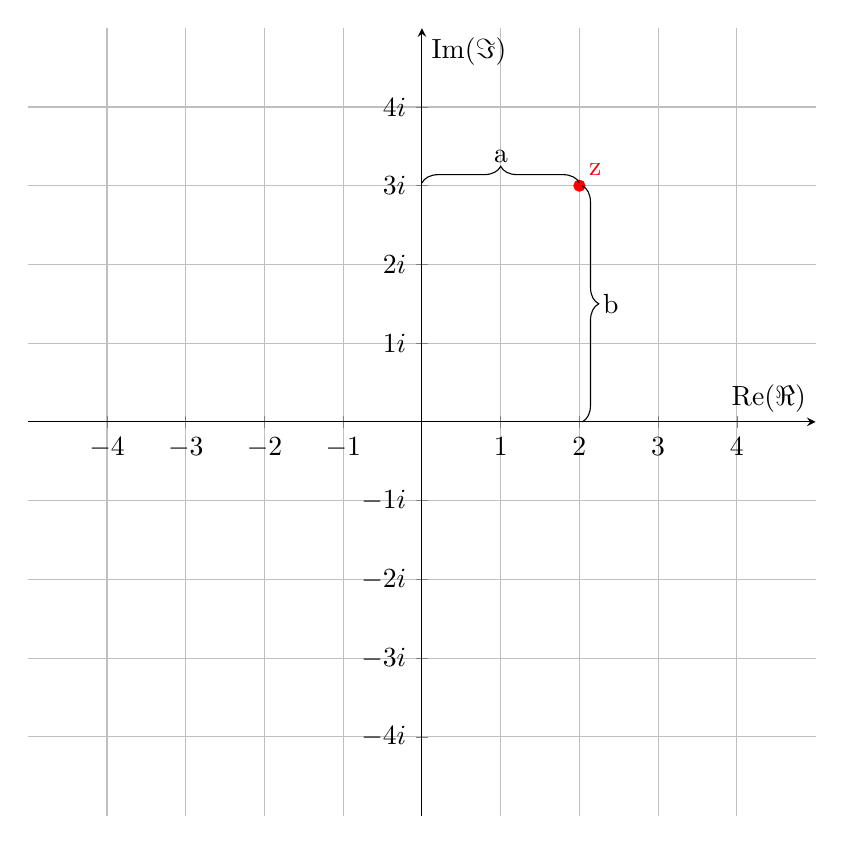
\begin{tikzpicture}
        \begin{axis}[
            samples=100,
            axis lines=center,
            x=1cm,
            y=1cm,
            xmin=-5, xmax=5,
            ymin=-5, ymax=5,
            xtick={-4, -3,...,3, 4},
            ytick={-4, -3,...,3, 4},
            xticklabels={$-4$,$-3$,$-2$,$-1$,$0$,$1$,$2$,$3$,$4$},
            yticklabels={$-4i$,$-3i$,$-2i$,$-1i$,$0i$,$1i$,$2i$,$3i$,$4i$},
            xlabel=$\mbox{Re} (\Re)$,
            ylabel=$\mbox{Im} (\Im)$,
            grid=major,
        ]

        \draw[color = red, fill] (2, 3) circle[radius=2pt, fill] node[above right]{ z };
        
        \draw[decorate, decoration = {brace,amplitude=6pt,raise=1pt}] (0, 3) -- (2, 3) node[midway, above, yshift=5pt]{a};
        \draw[decorate, decoration = {brace,amplitude=6pt,raise=1pt,mirror}] (2, 0) -- (2, 3) node[midway, right, xshift=5pt]{b};

        \end{axis}
    \end{tikzpicture}
}
\end{center}



    \subsection{Sind die reellen Zahlen wirklich eine Teilmenge von den komplexen Zahlen?}

    \parbox{0.9\textwidth}
{
    Nun haben wir eine neue Menge, in der $\mathbf{\sqrt{-1} = i}$ ist, jedoch
    wollen wir nun beweisen, dass die Menge eine \textbf{Erweiterung der reellen Zahlen} $\mathbb{R}$ ist.
    Dazu nutzen wir unsere vorherige Definition, laut der $\mathbf{x \cdot 1 = \left(x; 0\right)}$ ist,
    nun nehmen wir zwei Zahlen $\mathbf{a}$, $\mathbf{b}$ mit $\mathbf{a, b \in \mathbb{R}}$, schreiben
    sie nach Definition auf: $\mathbf{a \cdot 1 = \left(a; 0\right)}$ und $\mathbf{b \cdot 1 = \left(b; 0\right)}$
    und addieren sie $\mathbf{a \cdot 1 + b \cdot 1 = \left(a + b\right) \cdot 1}$ und
    $\mathbf{\left(a; 0\right) + \left(b; 0\right) = \left(a + b; 0\right) = \left(a + b\right) \cdot 1}$
    beim Vergleichen, stellen wir fest, dass die beiden Ergebnisse \textbf{gleich} sind, dass bedeutet,
    dass alle Elemente aus $\mathbf{\mathbb{C}}$ mit $\mathbf{(a \cdot 1) \in \mathbb{R}}$ sich \textbf{gleich wie
    die Reellen Zahlen verhalten}. \\

    Wir schreiben also $z=(a;b)=a\mathbf{1}+b\mathbf{i}$, jedoch verzichten wir auf
    die $\mathbf{1}$ und schreiben $\mathbf{i}$ ohne Fettdruck, also $z = (a;b) = a + b \cdot i$.
}

    %\newpage

    %\subsection{Arithmetik}

    %\begin{tabular}{c|c}
    \parbox{0.45\textwidth}
    {
        \begin{alignat*}{3}
            &z_1 + z_2 &&= (a + bi) + (c + di) = (a + c) + (b + d)i \\
        \end{alignat*}
    }
    &
    \parbox{0.45\textwidth}
    {
        \begin{alignat*}{3}
            &\left(a; b\right) + \left(c; d\right) &&= \left(a + c; b + d\right) \\
            &\left(a; b\right) - \left(c; d\right) &&= \left(a - c; b - d\right) \\
            &\left(a; b\right) \cdot \left(c; d\right) &&= \left(ac - bd; ad + bc\right) \\
            &\,\,r \cdot \left(a; b\right) &&= \left(ra; rb\right) \qquad r \in \mathbb{R} \\
        \end{alignat*}
    }
\end{tabular}

    \subsection{Aufgaben}

    \subsubsection{Berechnen Sie:}

\begin{enumerate}[label=\alph*)]
    \item $\left(5; 4\right) - \left(1; -2\right)$
    \item $3 \cdot \left(2; -1\right)$
    \item $\left(6; 0\right) \cdot \left(4; 1\right)$
    \item $\left(1; 3\right) \cdot \left(1; -3\right)$
    \item Berechnen Sie die ersten drei Potenzen von $\left(2; -2\right)$.
\end{enumerate}

\subsubsection{Bestimmen Sie Real- und Imaginärteil von: }

\begin{enumerate}[label=\alph*)]
    \item $z = \left(2 - 7i\right) + \left(12 - 13i\right)$
    \item $z = \left(5 + 7i\right) \cdot \left(3 + i\right)$
\end{enumerate}


\subsubsection{Benutze $i = \left(0;1\right)$ um $i^2 = - 1$ nachzuweisen}

\subsubsection{Bestimmen Sie die reelen Zahlen $c$ und $d$ so, dass $\left(-1; 2\right) \cdot \left(c; d\right) = \left(-13; 1\right)$}

\subsubsection{Beweise, dass für $a \cdot b$, das Kommutativgesetz gilt}
\subsubsection{Beweise, dass für $a \cdot b$, das Distributivgesetz gilt}


\end{document}